\documentclass[12pt]{article}

\usepackage{array}
\usepackage{algorithm}
\usepackage{algpseudocode}
\usepackage{amsmath}
\usepackage{amsfonts}
\usepackage{float}
\usepackage{fancyhdr}
\usepackage{graphicx}
\usepackage{placeins}
\usepackage[colorlinks=true,linkcolor=blue, citecolor=red]{hyperref}
\usepackage{url}
\usepackage[top=.75in, left=.75in, right=.75in, bottom=1in]{geometry}
\usepackage{arydshln}
\usepackage[utf8]{vietnam}
\usepackage{listings}

\usepackage{xcolor}

%New colors defined below
\definecolor{codegreen}{rgb}{0,0.6,0}
\definecolor{codegray}{rgb}{0.5,0.5,0.5}
\definecolor{codepurple}{rgb}{0.58,0,0.82}
\definecolor{backcolour}{rgb}{0.95,0.95,0.92}

%Code listing style named "mystyle"
\lstdefinestyle{mystyle}{
  backgroundcolor=\color{backcolour}, commentstyle=\color{codegreen},
  keywordstyle=\color{magenta},
  numberstyle=\tiny\color{codegray},
  stringstyle=\color{codepurple},
  basicstyle=\ttfamily\footnotesize,
  breakatwhitespace=false,         
  breaklines=true,                 
  captionpos=b,
  escapeinside={\%*}{*)},
  keepspaces=true,                 
  numbers=left,                    
  numbersep=5pt,                  
  showspaces=false,                
  showstringspaces=false,
  showtabs=false,                  
  tabsize=2
}


\setlength{\headheight}{29.43912pt}
\setlength{\parindent}{0pt}

\usepackage{mathptmx}
% \graphicspath{PATH_TO_GRAPHIC_FOLDER}

\newcommand{\reporttitle}{Báo cáo Đồ án Môn học}
\newcommand{\coursename}{Khai thác ngữ liệu văn bản nâng cao (MTH089)}
\newcommand{\reportname}{Xây dựng ứng dụng trích xuất triệu chứng sử dụng mô hình ViHealthBERT}


\pagestyle{fancy}
\fancyfoot{}
\fancyfoot[R]{Page \thepage}

\lhead{
\reporttitle
}
\rhead{
Trường Đại học Khoa học Tự nhiên - ĐHQG HCM\\
Khai thác ngữ liệu văn bản nâng cao (MTH089)
}
\lfoot{\LaTeX\ template by \href{https://github.com/trhgquan}{Quan, Tran Hoang}}

\begin{document}
\begin{titlepage}
\newcommand{\HRule}{\rule{\linewidth}{0.5mm}}
\centering

\textsc{\LARGE đại học quốc gia tphcm}\\[1.5cm]
\textsc{\Large trường đại học khoa học tự nhiên}\\[0.5cm]
\textsc{\large khoa công nghệ thông tin}\\[0.5cm]
% \textsc{bộ môn công nghệ tri thức}\\[0.5cm]

\HRule \\[0.4cm]
{ 
\huge{\bfseries{\reporttitle}}\\[0.5cm]
\large{\bfseries{Đề tài: \reportname}}
}\\[0.4cm]
\HRule \\[0.5cm]

\textbf{\large Môn học: \coursename}\\[0.5cm]

\begin{minipage}[t]{0.4\textwidth}
\begin{flushleft} \large
\emph{Học viên thực hiện:}\\
Trần Hoàng Quân (19120338) \\
Phạm Anh Việt \textsc{(20C11060)} \\
Nguyễn Đức Thuận \textsc{(21C11035)} \\
Nguyễn Thiện Dương \textsc{(21C12004)} \\
\end{flushleft}
\end{minipage}
~
\begin{minipage}[t]{0.4\textwidth}
\begin{flushright} \large
\emph{Giáo viên hướng dẫn:} \\
% Dr. James \textsc{Smith}
TS. Nguyễn Trường Sơn\\
TS. Nguyễn Tiến Huy
\end{flushright}
\end{minipage}\\[1cm]

{\large \today}\\[1cm]


\includegraphics[scale=.3]{img/hcmus-logo.png}\\[1cm] 

\vfill
\end{titlepage}
\tableofcontents
\pagebreak



\section{Mô hình ViHealthBERT}
\subsection{Tóm tắt nội dung bài báo}
Trong những năm gần đây, các mô hình ngôn ngữ (Language Models - LM) được xây dựng và ứng dụng rộng rãi trong lĩnh vực Xử lý ngôn ngữ tự nhiên (NLP), chúng cũng đạt được nhiều kết quả đáng chú ý. Đặc biệt, chất lượng các mô hình đơn ngữ được huấn luyện sẵn dành cho những ngôn ngữ ít tài nguyên ngữ liệu đã tăng đáng kể. Đáng lưu ý, mặc dù các mô hình ngôn ngữ cho miền chung (general-domain language models) rất đa dạng, nhưng có rất ít các mô hình ngôn ngữ đặc thù dành riêng cho một số lĩnh vực (specific-domain language models). Vì lí do đó, nhóm tác giả bài báo \textit{ViHealthBERT: Pre-trained Language Models for Vietnamese in Health Text Mining}\cite{minh-EtAl:2022:LREC} công bố bài báo với những đóng góp sau:
\begin{itemize}
\item Giới thiệu mô hình ViHealthBERT là mô hình ngôn ngữ Tiếng Việt đặc thù cho lĩnh vực y tế.
\item Giới thiệu các bộ ngữ liệu Acronym Disambiguation (AD) và Freqently Asked Question (FAQ) Summarization là các bộ ngữ liệu đặc thù cho lĩnh vực y tế.
\end{itemize}

\subsection{Kiến trúc mô hình ViHealthBERT}
\subsubsection{Transformer và BERT}
Mô hình Transformer ứng dụng cơ chế self-attention và multi-head attention được giới thiệu lần đầu trong paper Attention is All You Need\cite{DBLP:journals/corr/VaswaniSPUJGKP17}. 
\begin{figure}
\centering
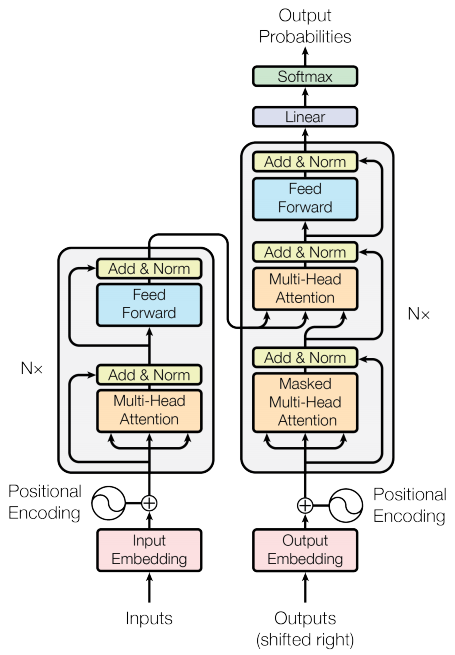
\includegraphics[scale=.35]{img/transformer.png}
\caption{Kiến trúc Transformer\cite{DBLP:journals/corr/VaswaniSPUJGKP17}}
\label{fig:transformer_diagram}
\end{figure}
Phần Encoder của Transformer được sử dụng trong mô hình BERT (\textbf{B}idirectional \textbf{E}ncoder \textbf{R}epresentations from \textbf{T}ransformers)\cite{devlin-etal-2019-bert}. Trong bài báo, BERT được giới thiệu có 2 phiên bản với các siêu tham số (hyperparameters) và số lượng tham số huấn luyện (training parameters) khác nhau:
\begin{itemize}
\item \textbf{BERT\textsubscript{base}}: 12 Transformer encoder layers, 768 hidden units, 12 attention heads, 110 triệu parameters.
\item \textbf{BERT\textsubscript{large}}: 24 Transformer encoder layers, 1024 hidden units, 16 attention heads và 340 triệu parameters.
\end{itemize}
\begin{figure}
\centering
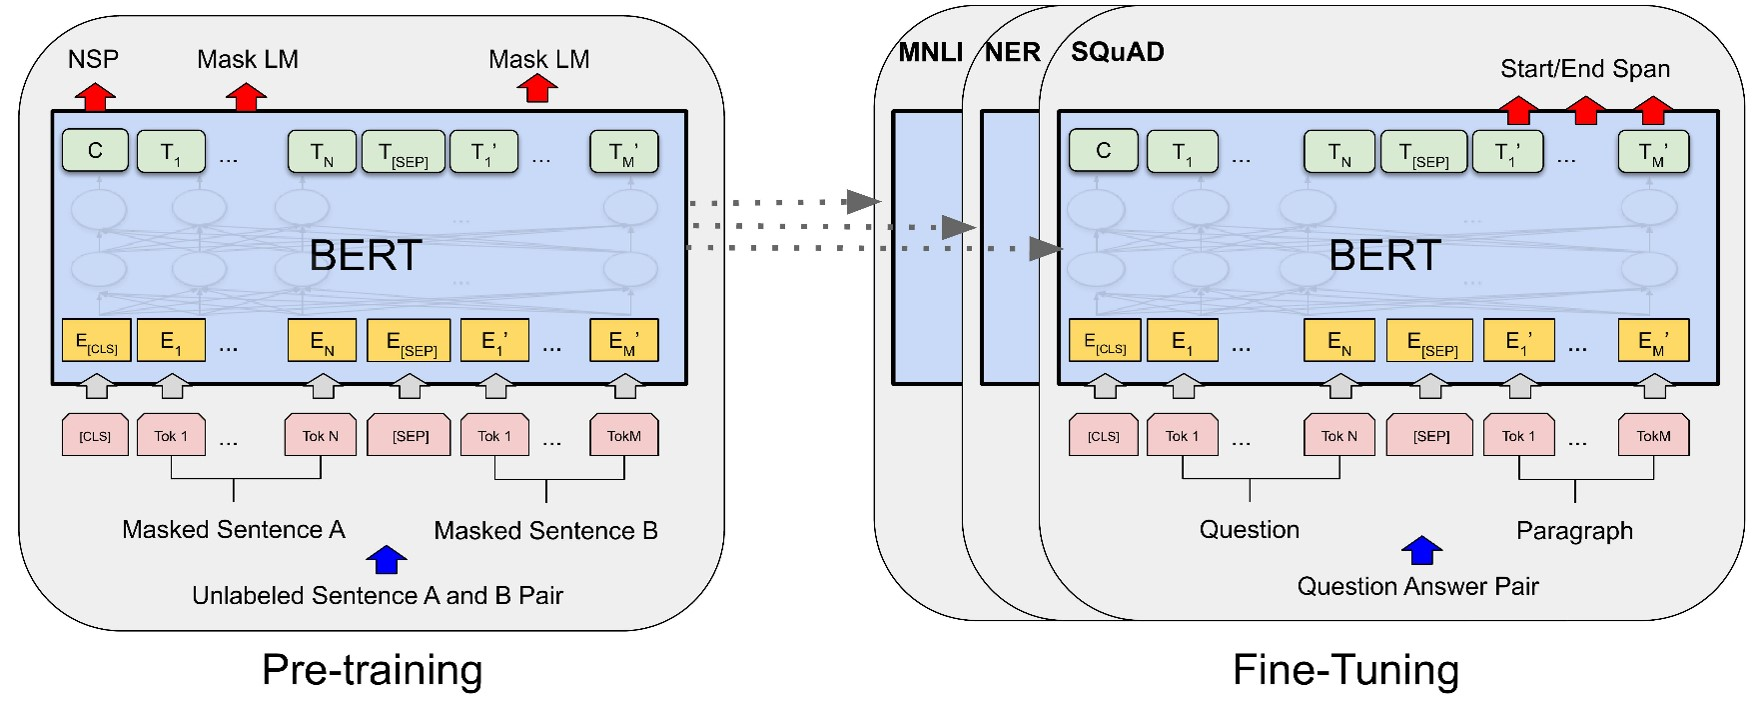
\includegraphics[scale=.65]{img/BERT.jpg}
\caption{Mô hình BERT\cite{devlin-etal-2019-bert}}
\label{fig:my_label}
\end{figure}
BERT được tiền huấn luyện (pretraining) với bộ ngữ liệu \textit{BookCorpus} (800 triệu từ) và \textit{Wikipedia English} (2500 triệu từ), sau đó tinh chỉnh (finetune) lại cho từng task khác nhau. Sau khi BERT được công bố, nhiều mô hình cải tiến của BERT cũng được giới thiệu dựa trên kiến trúc của BERT, trong đó có thể kể đến
\begin{itemize}
\item \textbf{RoBERTa} (\textbf{R}obustly \textbf{o}ptimized \textbf{BERT} Pretraining \textbf{a}pproach)\cite{DBLP:journals/corr/abs-1907-11692}: sử dụng dynamic masking so với sử dụng static masking trong kiến trúc gốc; huấn luyện trên nhiều ngữ liệu hơn.
\item \textbf{DistilBERT}\cite{DBLP:journals/corr/abs-1910-01108}: mô hình nhỏ, nhanh, tốn ít chi phí huấn luyện hơn mô hình BERT gốc: có ít hơn 40\% parameters, chạy nhanh hơn 60\% nhưng hiệu quả bằng 95\% so với mô hình gốc.
\end{itemize}

\subsubsection{PhoBERT}
Dựa trên mô hình BERT, nhóm nghiên cứu từ VinAI đã công bố PhoBERT\cite{phobert}, được giới thiệu là mô hình ngôn ngữ đơn ngữ dành cho tiếng Việt có quy mô lớn đầu tiên. PhoBERT sử dụng quá trình pretraining của RoBERTA để tăng hiệu quả cho mô hình. Kiến trúc của PhoBERT vẫn giữ nguyên so với BERT:
\begin{itemize}
\item \textbf{PhoBERT\textsubscript{base}}: 12 encoder layers, 768 hidden units, 12 attention heads, 135 triệu parameters.
\item \textbf{PhoBERT\textsubscript{large}}: 24 encoder layers, 1024 hidden units, 16 attention heads và 370 triệu parameters.
\end{itemize}
PhoBERT được pretrain với bộ ngữ liệu \textit{Wikipedia Tiếng Việt} và bộ ngữ liệu tin tức tiếng Việt \textit{Binhvq News Corpus}

\subsubsection{ViHealthBERT}
Mô hình ViHealthBERT sử dụng kiến trúc của BERT (12 encoder layer, 768 hidden units, 12 attention heads) với bộ trọng số huấn luyện của PhoBERT. Việc huấn luyện ViHealthBERT chia làm 2 giai đoạn:
\begin{itemize}
\item \textbf{Giai đoạn pretraining}: Huấn luyện trên các bộ ngữ liệu \textit{Text Mining Corpus} và \textit{OSCAR} : Masked Language Modeling (MLM), Capitalized Prediction (CP) và Next Sentence Prediction (NSP).
\item \textbf{Giai đoạn finetuning}: Finetuning trên các bộ ngữ liệu \textit{PhoNER\_COVID-19, VimQ, arcDrid} và \textit{FAQ Summarization}: Named-Entity Recognition (NER), Acronym Disambiguation và FAQ Summarization
\end{itemize}
\begin{figure}
\begin{center}
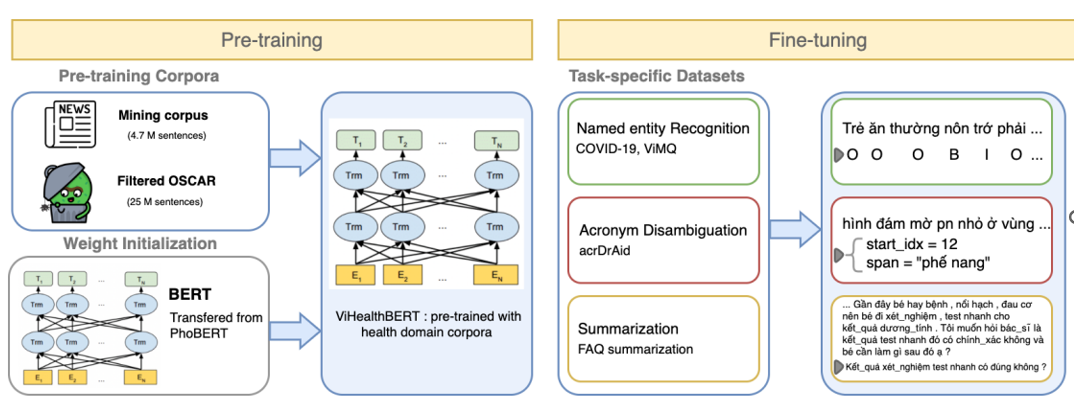
\includegraphics[scale=.8]{img/ViHealthBERT.png}
\caption{Tổng quan về quá trình pretraining và finetuning trong ViHealthBERT\cite{minh-EtAl:2022:LREC}}
\end{center}
\end{figure}
\section{Ứng dụng mô hình ViHealthBERT xây dựng công cụ trích xuất danh sách triệu chứng từ miêu tả của bệnh nhân}
\subsection{Động lực}
Một số bệnh viện có thiết lập hệ thống tư vấn bệnh trực tuyến: người bệnh gửi thông tin cá nhân cùng miêu tả triệu chứng, bác sĩ sẽ đọc và đưa ra chẩn đoán dựa trên miêu tả của người bệnh. Tuy nhiên, đôi khi người bệnh đưa ra nhiều thông tin không liên quan, trong khi bác sĩ chỉ cần danh sách các triệu chứng cụ thể để biết được bệnh nhân đang gặp vấn đề gì, từ đó đưa ra chẩn đoán phù hợp.

Nhóm đề xuất sử dụng mô hình ViHealthBERT ứng dụng vào bài toán Medical Named Entity Recognition (Medical NER) Tiếng Việt để tự động trích xuất danh sách các triệu chứng từ miêu tả của bệnh nhân, giúp tăng hiệu suất làm việc ở các cơ sở khám chữa bệnh.

\subsection{Finetune mô hình ViHealthBERT cho tác vụ NER}
\subsubsection{Ngữ liệu huấn luyện}
Nhóm tiến hành finetune lại mô hình ViHealthBERT để giải quyết bài toán Medical NER Tiếng Việt trên tập ngữ liệu PhoNER\_COVID19\cite{truong-etal-2021-covid}. Bộ ngữ liệu có các thông số được trình bày trong bảng~\ref{tab:covid-ner-vietnamese-stats}
\begin{table}
\centering
\begin{tabular}{|l|l|l|l|l|l|}
\hline
\textbf{Entity type} & \textbf{Train} & \textbf{Valid} & \textbf{Test} & \textbf{All} \\
\hline
PATIENT\_ID & 3240 & 1276 & 2005 & 6521 \\
\hdashline
PERSON\_NAME & 349 & 188 & 318 & 855 \\
\hdashline
AGE & 682 & 361 & 582 & 1625 \\
\hdashline
GENDER & 542 & 277 & 462 & 1281 \\
\hdashline
OCCUPATION & 205 & 132 & 173 & 510 \\
\hdashline
LOCATION & 5398 & 2737 & 4441 & 12576 \\
\hdashline
ORGANIZATION & 1137 & 551 & 771 & 2459 \\
\hdashline
SYMPTOM \& DISEASE & 1439 & 766 & 1136 & 3341 \\
\hdashline
TRANSPORTATION & 226 & 87 & 193 & 506 \\
\hdashline
DATE & 2549 & 1103 & 1654 & 5306 \\
\hline
\# Entities in total & 15767 & 7478 & 11735 & 34984 \\
\hline
\# Sentences in total & 5027 & 2000 & 3000 & 10027 \\
\hline
\end{tabular}
\caption{Các thông số của tập ngữ liệu PhoNER\_COVID19\cite{truong-etal-2021-covid}}
\label{tab:covid-ner-vietnamese-stats}
\end{table}

\subsubsection{Thông số huấn luyện và kết quả}
Nhóm tác giả huấn luyện ViHealthBERT cho tác vụ NER bằng cách sử dụng pretraining weight của ViHealthBERT và
\begin{itemize}
\item Dựng một layer classifier đơn giản (Linear + Dropdown) hoặc
\item Sử dụng một layer Conditional Random Field (CRF).
\end{itemize}
Ở đây nhóm tiến hành finetune ViHealthBERT theo cách đầu tiên, dựng một classifier layer đơn giản. Các thông số huấn luyện được mô tả trong bảng~\ref{tab:configurations}. Nhóm sử dụng các độ đo Precision, Recall và F1-Score để đánh giá kết quả huấn luyện. Với \textit{TP} là số lượng mẫu đúng được dự đoán đúng (True Positive), \textit{FP} là số lượng mẫu đúng nhưng được dự đoán sai (False Positive) và \textit{FN} là số lượng mẫu sai và được dự đoán sai (False Negative). Công thức tính Precision, Recall và F1-Score được định nghĩa như sau:
\begin{equation*}
\begin{aligned}
Precision (P) &= \frac{TP}{TP + FP} \\
Recall (R) &= \frac{TP}{TP + FN} \\
F1 &= \frac{2PR}{P + R}
\end{aligned}
\end{equation*}

Mô hình sau khi huấn luyện đạt được 95\% Precision, 94\% Recall và 95\% F1-Score khi đối chiếu với tập test của bộ ngữ liệu PhoNER\_COVID-19 đã nhắc ở phần trên. Kết quả huấn luyện của mô hình được mô tả trong bảng~\ref{tab:results-test}.
\begin{table}
\centering
\begin{tabular}{|l|c|}
\hline
\# epochs & 10 \\
\hline
batch size & 16 \\
\hline
seqlen & 70 \\
\hline
learning rate & 5e-5 \\
\hline
dropout rate & 0.1 \\
\hline
\end{tabular}
\caption{Thông số finetune mô hình ViHealthBERT cho tác vụ NER}
\label{tab:configurations}
\end{table}

\begin{table}
\centering
\begin{tabular}{|l|l|l|l|}
\hline
\textbf{label}        & \textbf{precision} & \textbf{recall} & \textbf{f1-score} \\ \hline
DATE                  & 0.9909             & 0.9921          & 0.9915            \\ \hdashline
SYMPTOM\_AND\_DISEASE & 0.9322             & 0.9040          & 0.9179            \\ \hdashline
NAME                  & 0.9073             & 0.9073          & 0.9073            \\ \hdashline
LOCATION              & 0.9529             & 0.9381          & 0.9454            \\ \hdashline
PATIENT\_ID           & 0.9857             & 0.9841          & 0.9849            \\ \hdashline
TRANSPORTATION        & 0.9442             & 0.9637          & 0.9538            \\ \hdashline
GENDER                & 1.0000             & 0.9776          & 0.9887            \\ \hdashline
ORGANIZATION          & 0.9064             & 0.9182          & 0.9123            \\ \hdashline
JOB                   & 0.8659             & 0.8208          & 0.8427            \\ \hdashline
AGE                   & 0.9803             & 0.9681          & 0.9741            \\ \hline
\textbf{micro avg}    & 0.9592             & 0.9497          & 0.9545            \\ \hline
\textbf{macro avg}    & 0.9592             & 0.9497          & 0.9544            \\ \hline
\end{tabular}
\caption{Kết quả finetune mô hình ViHealthBERT cho tác vụ NER trên tập test của bộ ngữ liệu PhoNER\_COVID-19}
\label{tab:results-test}
\end{table}

\subsection{Xây dựng ứng dụng}
Ứng dụng cần nhận biết và trích xuất các triệu chứng bệnh từ đầu vào là văn bản của người dùng. Do vậy, nhóm sẽ trích xuất các từ được gán nhãn \textit{SYMPTOM\_AND\_DISEASE} trong văn bản. Một ví dụ cho input (câu văn miêu tả triệu chứng) và output (danh sách các nhãn của câu) có thể thấy trong hình~\ref{fig:example-result}.

Từ mô hình đã huấn luyện, nhóm tiến hành xây dựng ứng dụng web cho phép người dùng nhập vào một câu văn (đoạn văn). Dữ liệu được đưa vào mô hình ViHealthBERT đã được finetune để gán nhãn, sau đó bộ nhãn và câu đầu vào sẽ được đưa vào một thuật toán đơn giản để trích ra danh sách các triệu chứng. Workflow của ứng dụng có thể được tóm tắt qua hình~\ref{fig:workflow}.
\begin{figure}
\centering
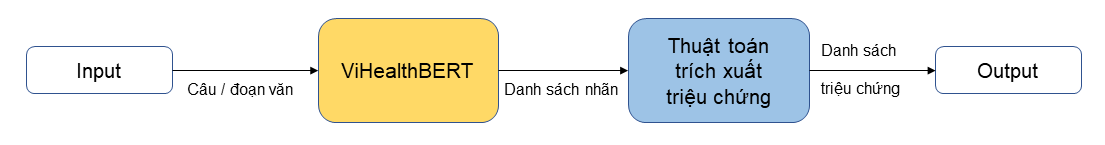
\includegraphics[scale=.6]{img/workflow.png}
\caption{Workflow ứng dụng trích xuất triệu chứng}
\label{fig:workflow}
\end{figure}
Cài đặt cụ thể của ứng dụng sẽ được nêu chi tiết ở các phần sau.

\subsubsection{VnCoreNLP và word segmentation}
 Với đầu vào là đoạn văn bản \texttt{text}, nhóm dùng công cụ VnCoreNLP\footnote{\href{https://github.com/vncorenlp/VnCoreNLP}{https://github.com/vncorenlp/VnCoreNLP}} để thực hiện tác vụ tách từ (word segmentation).

\lstset{style=mystyle}
\lstinputlisting[language=Python]{source/segmentation.py}
Ví dụ:
\begin{itemize}
\item \textbf{Input}: 
\textit{Thưa bác sĩ, bệnh nhân 911 nam 27 tuổi quốc tịch Việt Nam ho đờm, chóng mặt, buồn nôn bị tiêu chảy}
\item \textbf{Output}: Thưa bác\_sĩ , bệnh\_nhân 911 nam 27 tuổi quốc\_tịch Việt\_Nam ho đờm , chóng\_mặt , buồn\_nôn bị tiêu\_chảy
\end{itemize}

\subsubsection{AutoTokenizer}
Nhóm sử dụng tokenizer của ViHealthBERT để tokenize input. Theo code mẫu của nhóm tác giả:
\begin{itemize}
    \item \texttt{all\_input\_ids}: id của từng từ trong \texttt{input\_text}
    \item \texttt{all\_attention\_mask}: attention mask của từng từ trong \texttt{input\_text}
    \item \texttt{all\_slot\_labels\_ids}: id của từng nhãn cho mỗi từ.\footnote{Ngắn gọn hơn, đây là id của các nhãn NER.}
\end{itemize} 
Nhóm cũng đặt \texttt{max\_seq\_len = 70} - chiều dài tối đa của một sentence là 70 từ.
\lstset{style=mystyle}
\lstinputlisting[language=Python]{source/tokenizer.py}

\subsubsection{Layer classifier cho tác vụ NER}
Layer classifier cho tác vụ NER bao gồm 1 layer Linear và 1 layer Dropout:
\lstinputlisting[language=Python]{source/ner-layer.py}

\subsubsection{Kiến trúc ViHealthBERT cho tác vụ NER}
Kiến trúc ViHealthBERT cho tác vụ NER bao gồm 
\begin{itemize}
\item Backbone RoBERTa - PhoBERT.
\item Layer classifier \textbf{hoặc} layer Conditional Random Field (CRF). Nếu dùng layer classifier thì hàm loss sử dụng là CrossEntropy, ngược lại dùng CRF thì hàm loss sử dụng là hàm negative log-likelihood.
\end{itemize}

\lstinputlisting[language=Python]{source/vihealthbert.py}

\subsubsection{Khởi tạo model}
Khởi tạo model với pretrained weight của ViHealthBERT và dùng layer classifier với \texttt{dropout rate = 0.1}.
\lstinputlisting[language=Python]{source/init-model.py}

Output từ model sẽ là \texttt{label\_id} của từ tương ứng với các \texttt{slot\_labels\_ids} là các nhãn được định nghĩa từ trước:
\begin{lstlisting}[language=Python]
labels = ["O", "B-DATE", "I-DATE", "B-NAME", "B-AGE", "B-LOCATION", "I-LOCATION", "B-JOB", "I-JOB","B-ORGANIZATION", "I-ORGANIZATION", "B-PATIENT_ID", "B-SYMPTOM_AND_DISEASE", "I-SYMPTOM_AND_DISEASE","B-GENDER", "B-TRANSPORTATION", "I-TRANSPORTATION", "I-NAME", "I-PATIENT_ID", "I-AGE", "I-GENDER"]
\end{lstlisting}
Ví dụ:
\begin{itemize}
\item \textbf{Input}: \textit{Thưa bác sĩ, bệnh nhân 911 nam 27 tuổi quốc tịch Việt Nam ho đờm, chóng mặt, buồn nôn bị tiêu chảy.}
\item \textbf{Output}:
\vietnameselst
\lstinputlisting{source/json-output.json}
\end{itemize}

\subsubsection{Hàm trích xuất triệu chứng bệnh (tương ứng với label \textbf{SYMPTOM\_AND\_DISEASE}).}
Từ danh sách các từ và label tương ứng, ta tiến hành xây dựng một thuật toán đơn giản trích xuất các triệu chứng:
\lstinputlisting[language=Python]{source/symptom-extract.py}

\section{Hướng dẫn sử dụng ứng dụng}
\subsection{Clone project từ GitHub}
Tiến hành clone project từ GitHub:
\begin{lstlisting}
git clone git@github.com:AnhVietPham/DemoViHealthBERT-NER.git
\end{lstlisting}

\subsection{Cài đặt và khởi chạy server}
\begin{enumerate}
\item Cài đặt các thư viện cần thiết (Python):
\lstset{style=mystyle}
\begin{lstlisting}[language=bash]
pip install -r requirements.txt
\end{lstlisting}

\item Cài đặt Java SDK (yêu cầu phiên bản JDK / JRE ít nhất là v1.8)

\item Cài đặt VnCoreNLP cho quá trình pre-processing trước khi đưa dữ liệu vào mô hình để dự đoán.

\lstset{style=mystyle}
\begin{lstlisting}[language=bash]
bash vncorenlp.sh
\end{lstlisting}

\item Download model nhóm đã huấn luyện tại  \href{https://drive.google.com/drive/u/2/folders/19AGLo-27EeuXDkKG2JstuCgrcwB0854r}{link này}

\item Sau khi download model, ta giải nén model vào thư mục \texttt{model-save} sao cho cây thư mục của project có dạng như sau:
\lstinputlisting{source/dir-tree.txt}

\item Khởi chạy server
\lstset{style=mystyle}
\begin{lstlisting}[language=bash]
python main.py 
\end{lstlisting}
\end{enumerate}
\subsection{Cài đặt và khởi chạy phần ứng dụng web}
\begin{enumerate}
\item Cài đặt Flutter SDK (tham khảo tại \href{https://docs.flutter.dev/get-started/install}{link}).

\item Cập nhật phiên bản mới nhất của Flutter SDK.
\lstset{style=mystyle}
\begin{lstlisting}[language=bash]
flutter channel stable
flutter upgrade
\end{lstlisting}

\item Liệt kê danh sách các device có thể sử dụng để chạy ứng dụng Flutter.
\begin{lstlisting}[language=bash]
flutter devices
\end{lstlisting}
Kết quả thực hiện câu lệnh ở hình~\ref{fig:flutter-devices}. Ở đây nhóm sử dụng \texttt{chrome} trong danh sách connected devices, ngoài ra cũng có thể sử dụng \texttt{edge} hoặc các thiết bị mobile (nếu có).

\item Chạy ứng dụng Web.
\begin{lstlisting}[language=bash]
cd web-demo-ner
flutter run -d chrome
\end{lstlisting}
\end{enumerate}

\subsection{Demo}
Giao diện của ứng dụng sau khi khởi động sẽ như hình~\ref{fig:web-demo}. Với câu đầu vào \textit{Thưa bác sĩ, bệnh nhân 911 nam 27 tuổi quốc tịch Việt Nam ho đờm, chóng mặt, buồn nôn
bị tiêu chảy}, kết quả của ứng dụng đưa ra sẽ như hình~\ref{fig:web-demo-result}
\\\\
Video demo của ứng dụng trên YouTube.
\section{Tổng kết}
Qua đồ án này, nhóm xin tổng kết lại các nội dung đã thực hiện:
\begin{itemize}
\item Nhóm finetune mô hình ViHealthBERT cho tác vụ NER dùng bộ ngữ liệu  PhoNER\_COVID-19. Mô hình sau khi finetune đạt được 95\% Precision, 94\% Recall và 95\% F1-Score khi đối chiếu với tập test của bộ ngữ liệu PhoNER\_COVID-19.

\item Từ mô hình đã huấn luyện, nhóm xây dựng một ứng dụng hỗ trợ trích xuất các triệu chứng bệnh từ mô tả của người dùng.
\end{itemize}
Trong tương lai, nhóm đề xuất một số hướng cải tiến ứng dụng nhằm mang lại hiệu quả và trải nghiệm tốt nhất cho người sử dụng. Một số hướng cải tiến nhóm đề xuất bao gồm:
\begin{itemize}
\item Hỗ trợ nhập liệu từ file. Khi đó hệ thống có thể trích xuất và đưa ra danh sách triệu chứng của nhiều bệnh nhân cùng lúc.

\item Xây dựng một module chẩn đoán bệnh dựa trên danh sách các triệu chứng. Danh sách triệu chứng hiện có sẽ được đưa qua một mạng neural đơn giản để đưa ra chẩn đoán nhanh. Tuy nhiên người bệnh vẫn cần tham khảo ý kiến của bác sĩ để có được chẩn đoán chính xác nhất.
\end{itemize}
\cleardoublepage
\phantomsection
\addcontentsline{toc}{section}{Tài liệu}
\bibliographystyle{apalike}
\bibliography{ref/sample}

\end{document}